\documentclass[12pt]{article}
\usepackage[czech]{babel}
\usepackage[utf8]{inputenc}
\usepackage[plainpages=false,pdfpagelabels,unicode]{hyperref}
\usepackage[pdftex]{graphicx}
\usepackage[margin=2cm, includefoot]{geometry}
\usepackage{wrapfig}

\begin{document}

\title{Praktikum z patologické fyziologie \\
Ikterus u laboratorního potkana}
\author{Marie Ostrá}
\maketitle

\section{Úvod}

\begin{wrapfigure}{r}{0.4\linewidth}
  \vspace{-20pt}
  \begin{center}
	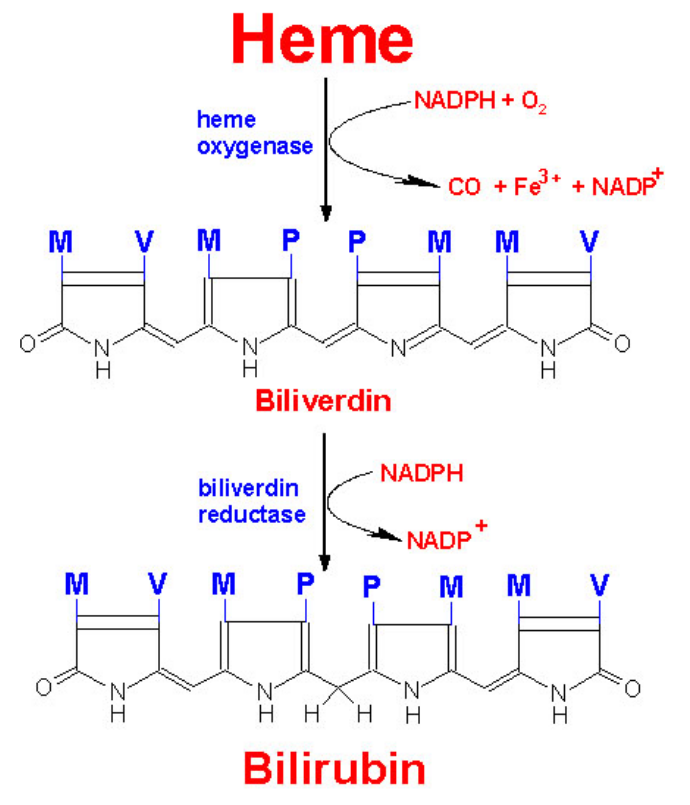
\includegraphics[width=\linewidth]{metabolismus-bilirubinu.png}
	\caption{Metabolismus hemu}
  \end{center}
  \vspace{-20pt}
\end{wrapfigure}

Ikterus (žloutenka) je žluté zabarvení kůže a sliznic způsobené zvýšenou hladinou bilirubinu v séru. Při mírném zvýšení nemusí být žluté zbarvení zřetelné (subikterus). Pro zvýšenou hladinu bilirubinu v séru se používá termín hyperbilirubinémie. Bilirubin je konečný produkt degradace hemu. Při zániku erytrocytů se z nich uvolňuje hemoglobin, z hemové části je hemoxygenázou odstraněno železo a zbytek je přeměněn na bilirubin. Další zpracování bilirubinu se děje výhradně v hepatocytech. Po vstupu do hepatocytu následuje jeho rychlá konjugace s glukuronovou kyselinou proti koncentračnímu gradientu do žluči. Vzniká ve vodě nerozpustný konjugovaný bilirubin.

\begin{figure}
	\begin{centering}
	
\includegraphics[width=0.6\linewidth]{bilirubin.png}
	\caption{Bilirubin}
	\end{centering}
\end{figure}

Podle mechanismu vzniku dělíme ikterus do tří skupin: prehepatální, hepatální a posthepatální. Prehepatální ikterus vzniká nadměrnou tvorbou bilirubinu při zvýšeném rozpadu erytrocytů (hemolytické anémie). Hepatocyty nestíhají konjugovat a vyloučit všechen bilirubin, zvyšuje se jeho hladina v séru a jeho ukládání v~tkáních způsobuje jejich žluté zbarvení. Hepatální ikterus je způsoben poruchou metabolizmu bilirubinu v játrech (vychytávání, konjugace nebo vylučování z hepatocytu) nebo poškozením až zánikem hepatocytů při jaterních chorobách. Příčinou vzniku posthepatálního ikteru je cholestáza (porucha odtoku žluči).

\section{Postup}
\subsection{Modelování obstrukčního ikteru podvazem ductus choledochus}
Laboratorního potkana zvážíme a uvedeme do celkové anestézie. Hmotnost si zaznamenáme.  Pomocí rozvěrače otevřemedutinu břišní a~najdeme játra, žaludek a duodenum, ve spojce jater a~duodena je spolu s venou portae ductus choledochus. Ductus choledochus opatrně oddělíme od vena portae a podvážeme.

Operační ránu uzavřeme ve dvou vrstvách. Další fáze pokusu následuje za týden.

\subsection{Diagnostika ikteru}
Potkana uvedeme obvyklým způsobem do narkózy. Porovnáme váhu zvířat před a po operaci, sledujeme zabarvení uší, paciček a ocasu a porovnáme s kontrolními zvířaty. Srdeční punkcí odebereme krev do stříkačky propláchnuté heparinem. Krev ze stříkačky (již bez jehly) opatrně vstříkneme do plastové zkumavky určené k centrifugaci. Po 10 minutách centrifugace (3000 otáček za minutu) získáme plazmu, kterou dále analyzujeme. Sledujeme zabarvení plazmy po centrifugaci. Punkcí močového měchýře odebereme moč. Pomocí indikátorových papírků vyšetříme přítomnost bilirubinu a urobilinogenu.

\newpage

\section{Výsledky}
\subsection{Hmotnost jater}

\begin{table}[h]
\begin{tabular}{|c|c|c|c|c|c|c|c|c|c|c|}
\hline
Rank Sum & Rank Sum & $U$ & $Z$ & $p$-value & $Z$ & $p$-value & Valid & Valid & 2*1sided \\
IK & KO & & & & adjusted & & $N$ IK & $N$ KO & exact $p$ \\
\hline
4194 & 177 & 122 & 3,628 & 0,000286 & 3,627564 & 0,000286 & 83 & 10 & 0,000101 \\
\hline
\end{tabular}
\caption{Mann-Whitney $U$ Test pro \% hmotnosti jater. Marked tests are significant at $p < 0,05$}
\end{table}

\begin{figure}[ht!]
	\begin{centering}
	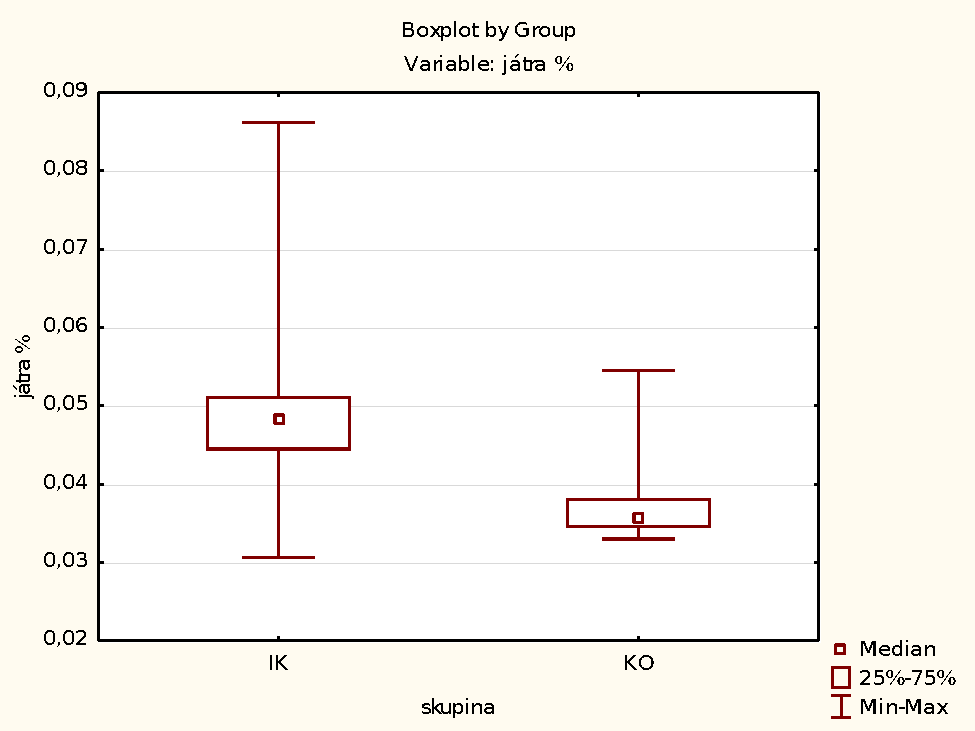
\includegraphics[width=\linewidth]{hmotnost-jatra.pdf}
	\caption{\% hmotnosti jater}
	\end{centering}
\end{figure}

\newpage

\subsection{Bilirubin celkový}

\begin{table}[h]
\begin{tabular}{|c|c|c|c|c|c|c|c|c|c|c|}
\hline
Rank Sum & Rank Sum & $U$ & $Z$ & $p$-value & $Z$ & $p$-value & Valid & Valid & 2*1sided \\
IK & KO & & & & adjusted & & $N$ IK & $N$ KO & exact $p$ \\
\hline
4043 & 52 & 7 & 4,8015 & 0,000002 & 4,8018 & 0,000002 & 81 & 9 & 0,000000 \\
\hline
\end{tabular}
\caption{Mann-Whitney $U$ Test pro celkový bilirubin. Marked tests are significant at $p < 0,05$}
\end{table}

\begin{figure}[ht!]
	\begin{centering}
	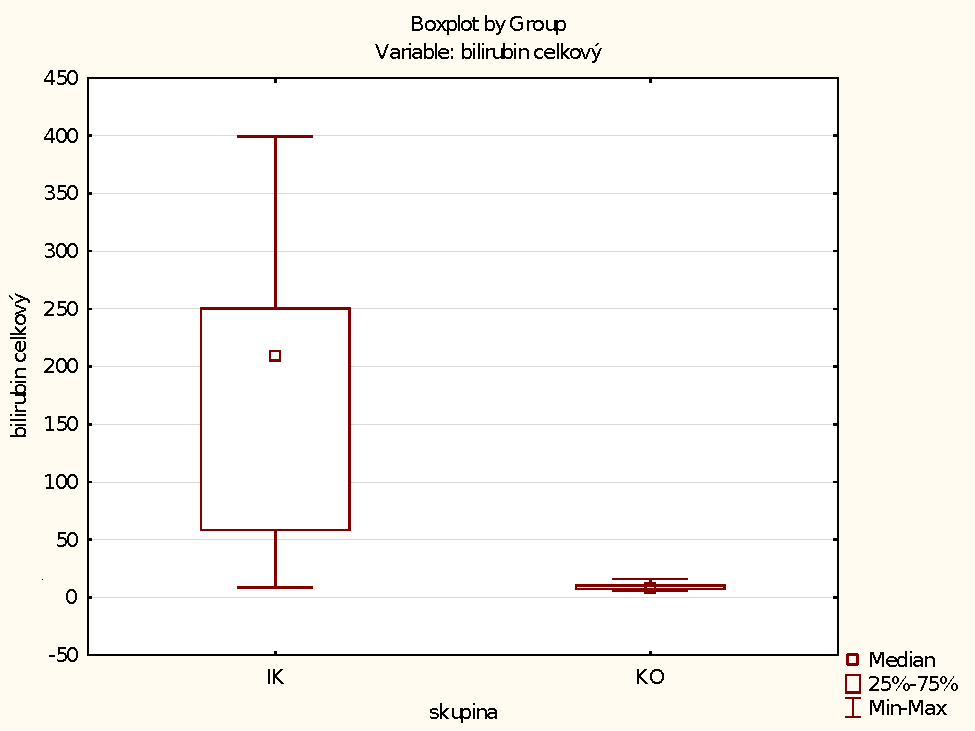
\includegraphics[width=\linewidth]{bilirubin-celkovy.pdf}
	\caption{Bilirubin celkový}
	\end{centering}
\end{figure}

\newpage

\subsection{Bilirubin přímý}

\begin{table}[h]
\begin{tabular}{|c|c|c|c|c|c|c|c|c|c|c|}
\hline
Rank Sum & Rank Sum & $U$ & $Z$ & $p$-value & $Z$ & $p$-value & Valid & Valid & 2*1sided \\
IK & KO & & & & adjusted & & $N$ IK & $N$ KO & exact $p$ \\
\hline
4044 & 51 & 6 & 4,8149 & 0,000001 & 4,8152 & 0,000001 & 81 & 9 & 0,000000 \\

\hline
\end{tabular}
\caption{Mann-Whitney $U$ Test pro bilirubin přímý. Marked tests are significant at $p < 0,05$}
\end{table}

\begin{figure}[ht!]
	\begin{centering}
	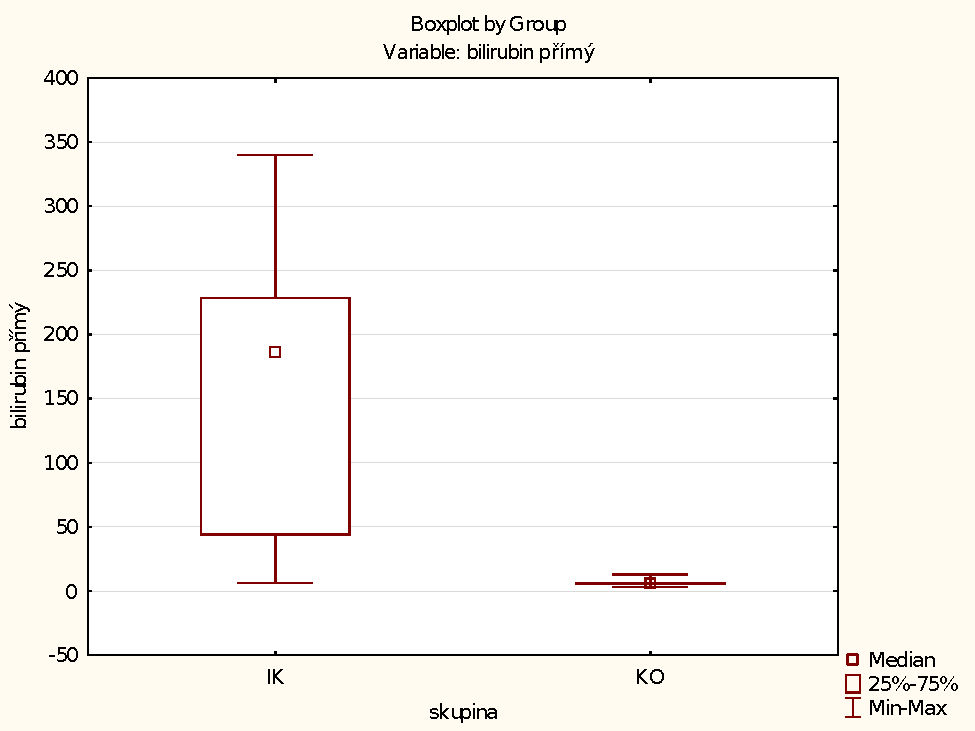
\includegraphics[width=\linewidth]{bilirubin-primy.pdf}
	\caption{Bilirubin přímý}
	\end{centering}
\end{figure}

\newpage

\subsection{Bilirubin nepřímý}

\begin{table}[h]
\begin{tabular}{|c|c|c|c|c|c|c|c|c|c|c|}
\hline
Rank Sum & Rank Sum & $U$ & $Z$ & $p$-value & $Z$ & $p$-value & Valid & Valid & 2*1sided \\
IK & KO & & & & adjusted & & $N$ IK & $N$ KO & exact $p$ \\
\hline
3987 & 108 & 63 & 4,0483 & 0,000052 & 4,0487 & 0,000052 & 81 & 9 & 0,000005\\
\hline
\end{tabular}
\caption{Mann-Whitney $U$ Test pro bilirubin nepřímý. Marked tests are significant at $p < 0,05$}
\end{table}

\begin{figure}[ht!]
	\begin{centering}
	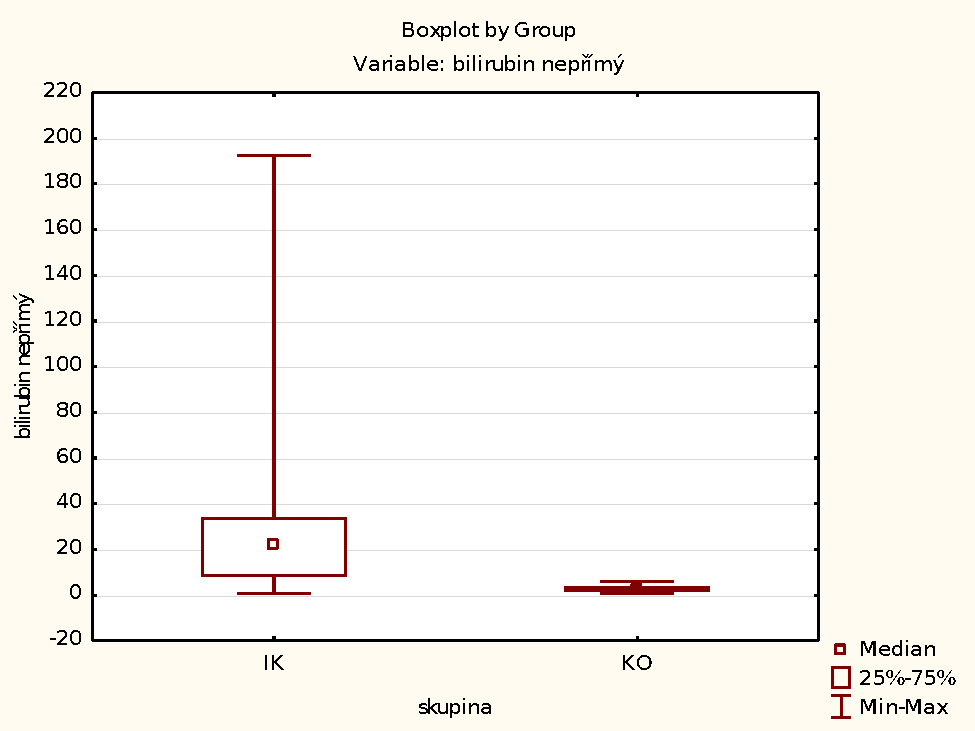
\includegraphics[width=\linewidth]{bilirubin-neprimy.pdf}
	\caption{Bilirubin nepřímý}
	\end{centering}
\end{figure}

\section{Závěr}
Praktikum proběhlo úspěšně. Podařilo se provést podvázání ductus choledochus a potkan zákrok přežil. Za týden od provedení zákroku byly na testovaném potkanovi vizuálně jasně patrné změny způsobené obstrukčním ikterem, tj. zabarvení paciček, uší a ocasu. Krom toho bylo dle očekávání pozorováno výrazné zvětšení hmotnosti jater a zvýšení koncentrace bilirubinu v séru.

\end{document}
